\documentclass[11pt]{beamer}

\usepackage[utf8]{inputenc}
\usepackage[T1]{fontenc}

% Graphics
\usepackage{graphicx}
\usepackage{tikz}
\usepackage{pgfplots}

% Language localization
\usepackage[swedish]{babel}

% Symbols
\usepackage{amsmath}
\usepackage{amsfonts}
\usepackage{amssymb}

% Bold math style, useful for vectors
\usepackage{bm}

\usepackage{ulem}

\usetheme{Madrid}
\setbeamertemplate{navigation symbols}{}

\begin{document}
	\author{Niklas Wingren}
	\title[Akusto-elektromagnetisk växelverkan]{Akusto-elektromagnetisk växelverkan i material}
	\subtitle{saker}
	\date{2019-01-15}
	\frame[plain]{\maketitle}
	
	\begin{frame}{Översikt}
		\tableofcontents
	\end{frame}
	
	\AtBeginSection[]{
		\begin{frame}{Översikt}
			\tableofcontents[currentsection]
		\end{frame}
	}
	
	\section{Bakgrund}
	
	\begin{frame}{Bakgrund}{Oförstörande provning}
		\begin{itemize}
			\item Elektromagnetiska och akustiska fenomen används separat inom oförstörande provning (OFP)
			\begin{itemize}
				\pause
				\item Ultraljudsmetoder etablerade sedan länge
				\pause
				\item Mikrovågs/mm-vågsavbildning relativt nytt
			\end{itemize}
			\pause
			\item Kombination kan ge mer information
			\pause
			\item Kunskap om möjliga interaktionsmekanismer krävs
		\end{itemize}
	\end{frame}
	
	\begin{frame}{Bakgrund}{Akusto-optik}
		\begin{columns}
			\begin{column}{0.6\textwidth}
				\begin{itemize}
					\item<1-> Interaktion mellan vågor i storleksordningarna ultraljud och optik
					\item<2-> Akustisk våg ger periodiskt störning i brytningsindex
					\item<3-> Konstruktiv interferens vid givet villkor (Braggvillkor)
					\begin{equation*}
						\sin{\theta_B} = \frac{\lambda}{2\Lambda}
					\end{equation*}
					\item<4-> Används inom fotonik för modulatorer, filter etc.
				\end{itemize}
			\end{column}
			\begin{column}{0.4\textwidth}
				\uncover<2->{
					\resizebox{\textwidth}{!}{
						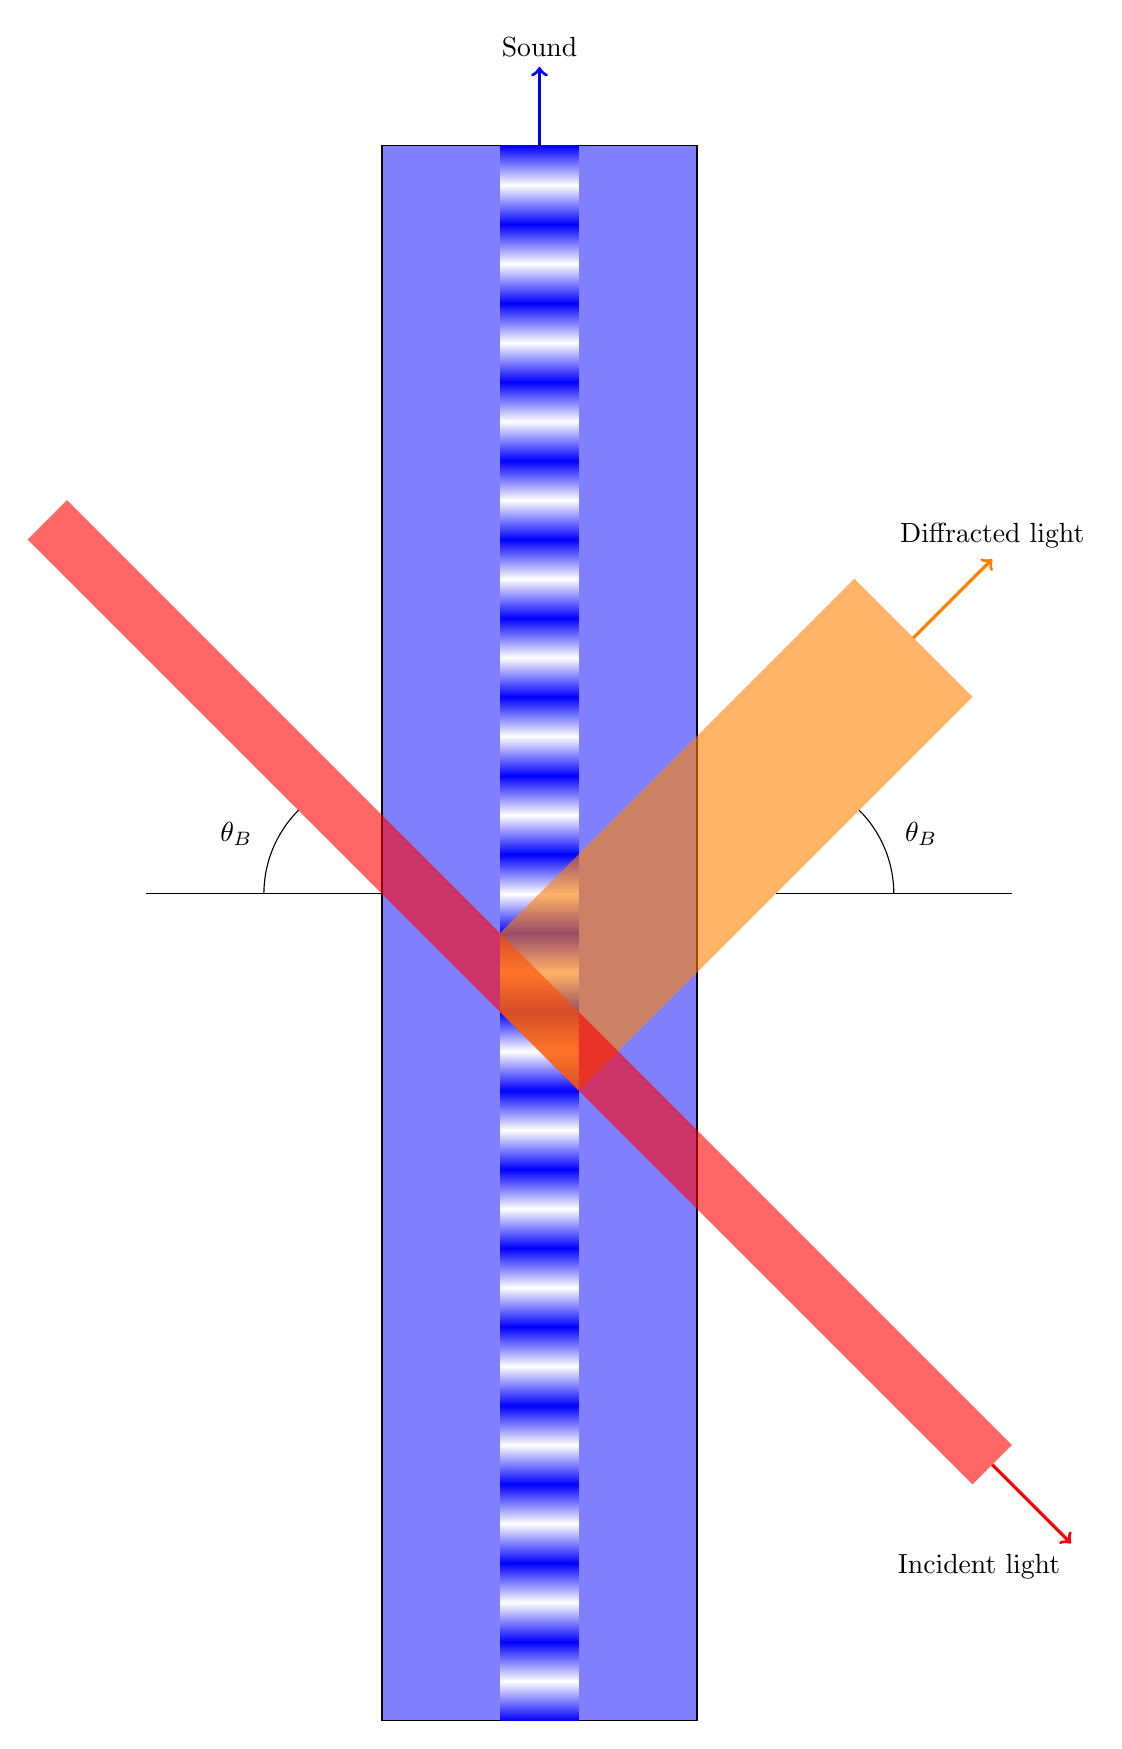
\begin{tikzpicture}
	\draw[fill=blue!50!white] (-2,0) rectangle ++(4,20);
	\foreach \i in {0,1,...,39}
		\path [bottom color=blue, top color=white, shading angle = {mod(\i,2)*180}]
		(-0.5,{\i/2}) rectangle ++(1,0.5);
		
	\fill[red,opacity=0.6] (-6.5,15) -- ++(7,-7) -- (0.5,9) -- ++({-7+sqrt(0.5-0.5*0.5)},7-0.5);
	\fill[orange,opacity=0.6] (0.5,8) -- ++(5,5) -- ++({-sqrt(4.5-1.5*1.5)},1.5) -- (-0.5,10) -- (-0.5,9);
	\fill[red,opacity=0.6] (0.5,8) -- ++(5,-5) -- ++({sqrt(0.5-0.5*0.5)},0.5) -- (0.5,9);
	
	\draw[->,blue,very thick] (0,20) -- (0,21) node[anchor=south,text=black]{Sound};
	\draw[->,orange,very thick] ({5.5-sqrt(4.5-1.5*1.5)+sqrt(1.5*1.5/2-0.75*0.75)},13.75) -- ++(1,1) node[anchor=south,text=black]{Diffracted light};
	\draw[->,red,very thick] ({5.5+sqrt(0.5-0.5*0.5)-sqrt(0.5*0.5/2-0.25*0.25)},3.25) -- ++(1,-1) node[anchor=north east,text=black]{Incident light};
	
	\draw (-2,10.5) -- ++(-3,0);
	\draw[shift={(-2,10.5)}] ([shift={(180:1.5)}] 0,0) arc(180:135:1.5) (157.5:2) node{$\theta_B$};
	\draw (3,10.5) -- ++(3,0);
	\draw[shift={(3,10.5)}] ([shift={(0:1.5)}] 0,0) arc(0:45:1.5) (22.5:2) node{$\theta_B$};
\end{tikzpicture}
					}
				}
			\end{column}
		\end{columns}
	\end{frame}
	
	\begin{frame}{Bakgrund}{RASS}
		\begin{itemize}
			\item Radio Acoustic Sounding System
			\pause
			\item Storleksordning MHz - GHz (EM) och hörbart ljud
			\pause
			\item Samma mekanism för interaktion som akusto-optik
			\pause
			\item Temperatur påverkar Braggvillkor genom akustisk våglängd
			\pause
			\item Används för att mäta temperaturprofiler i atmosfären
		\end{itemize}
	\end{frame}

	\begin{frame}{Bakgrund}{Lokaliserad harmonisk rörelse}
		\begin{itemize}
			\item<1-> Lokaliserad vibration genom akustisk strålningskraft
		\end{itemize}
		\begin{columns}
			\begin{column}{0.45\textwidth}
				\begin{itemize}
					\item<2-> Ultraljud amplitudmoduleras lokalt
					\item<3-> Elektromagnetisk frekvens skiftas med vibrationsfrekvens
				\end{itemize}
			\end{column}
			\begin{column}{0.3\textwidth}
				\uncover<2->{
					\resizebox{!}{0.5\textheight}{
						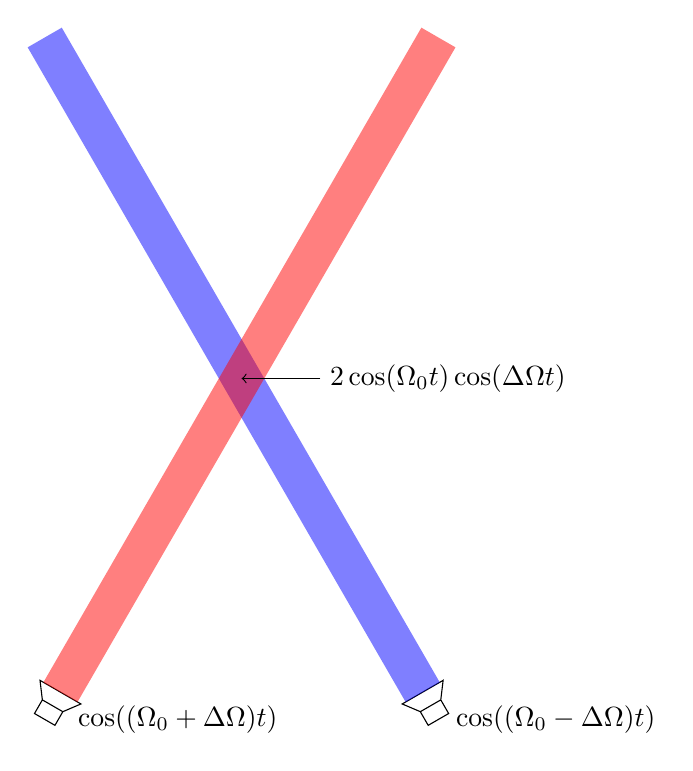
\begin{tikzpicture}
	% Blue beam
	\draw[shift={(2.5,0)},rotate={90+30}] (0,-0.15) rectangle (0.2,0.15) -- (0.4,0.3) -- (0.4,-0.3) -- (0.2,-0.15);
	\fill[blue,shift={(2.5,0)},rotate=30,opacity=0.5] (-0.25,0.4) rectangle (0.25,10);
	\draw (2.6,0) node[anchor=west]{$\cos((\Omega_0 - \Delta \Omega)t)$};
	
	% Red beam
	\draw[shift={(-2.5,0)},rotate={90-30}] (0,-0.15) rectangle (0.2,0.15) -- (0.4,0.3) -- (0.4,-0.3) -- (0.2,-0.15);
	\fill[red,shift={(-2.5,0)},rotate=-30,opacity=0.5] (-0.25,0.4) rectangle (0.25,10);
	\draw (-2.2,0) node[anchor=west]{$\cos((\Omega_0 + \Delta \Omega)t)$};

	\draw[->] (1,4.33) node[anchor=west]{$2\cos(\Omega_0 t)\cos(\Delta \Omega t)$} -- (0,4.33);
\end{tikzpicture}
					}
				}
			\end{column}
			\hspace{0.05\textwidth}
			\begin{column}{0.2\textwidth}
				\uncover<2->{
					\resizebox{!}{0.5\textheight}{
						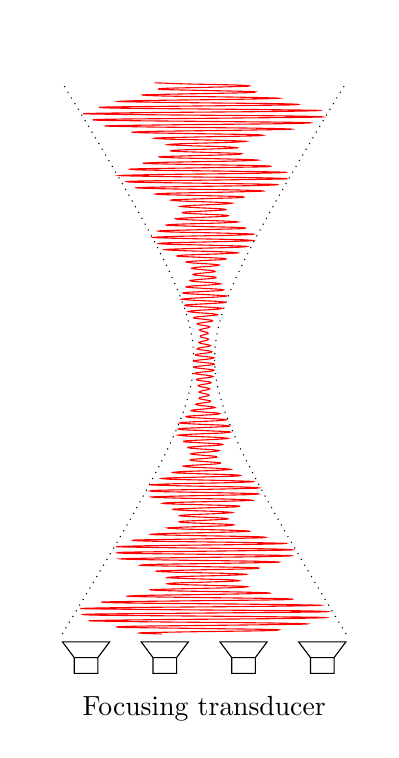
\begin{tikzpicture}
	% Draw array with 4 elements
	\foreach \x in {0,1,...,3}
		\draw[shift={({0.5+\x},0.2)},rotate={90}] (0,-0.15) rectangle (0.2,0.15) -- (0.4,0.3) -- (0.4,-0.3) -- (0.2,-0.15);
		
	\draw (2,-0.25) node{Focusing transducer};
		
	% Draw beam outline
	\begin{axis}[x=1cm,y=1cm,xticklabels={},yticklabels={},xmin=-2,xmax=2,axis line style={draw=none},tick style={draw=none}]
	\addplot[domain=0.5:7.5,smooth,variable=\y,dotted]  ({-2*sqrt(0.1+0.1*(\y-4)^2)+0.5},{\y});
	\addplot[domain=0.5:7.5,smooth,variable=\y,dotted]  ({2*sqrt(0.1+0.1*(\y-4)^2)-0.5},{\y});
	\addplot[domain=0.5:7.5,variable=\y,samples=500,smooth,red]  ({cos(\y*80 r)*(1+0.5*cos(\y*8 r))/1.5*(2*sqrt(0.1+0.1*(\y-4)^2)-0.5)},{\y});
	\end{axis} 
\end{tikzpicture}
					}
				}
			\end{column}
		\end{columns}
	\end{frame}
	
	\section{Teori}
	
	\begin{frame}{Teori}{Fotoelasticitet}
		content...
	\end{frame}
	
	\begin{frame}{Teori}{Spridning mot dielektrisk störning}
		content...
	\end{frame}

	\begin{frame}{Teori}{Radarekvation - plana vågor}
		content...
	\end{frame}

	\section{Numeriska simuleringar}
	
	\begin{frame}{Numeriska simuleringar}{Geometri}
		content...
	\end{frame}
	
	\begin{frame}{Numeriska simuleringar}{Svep av vinkel $\alpha$}
		content...
	\end{frame}
	
	\begin{frame}{Numeriska simuleringar}{Defekt med elektromagnetisk kontrast}
		content...
	\end{frame}
	
	\begin{frame}{Numeriska simuleringar}{Defekt med mekanisk kontrast}
		content...
	\end{frame}
	
	\section{Slutsatser}
	
	\begin{frame}{Slutsatser}
		content...
	\end{frame}

\end{document}
